%!TEX root=main.tex
\subsection{Descripción del SAI}

El SAI se define como un sistema de ensamble vertical de tres componentes, organizados para ajustarse entre sí y formar un Conjunto Contenedor, el SAI consta de dos Envases Individuales Dosificadores de productos líquidos o aceites comestibles los cuales incorporan un Atomizador para la dosificación de su contenido, estos envases son ensamblados por el tercer componente: Tapa Doble de Soporte interpuesta entre dichos envases individuales acoplados coaxial e invertidamente de forma vertical, que también funciona como un envase dosificador de especies en grano.

Este Conjunto Contenedor tiene la condición de Objeto de Invención (otorgada por la patente de INAPI N$^{o}$50.295, 22/10/2009) al desarmarse en componentes individuales como utensilios de cocina, y armarse en su forma integrada que permite que sus componentes se ajusten perfectamente formando un solo volumen que se puede manejar en forma inversa, para cambiar y elegir el envase que se desea utilizar.


\subsection{Sobre la propiedad intelectual}

La propiedad intelectual es una rama del derecho que fomenta la innovación, la creación y la transferencia tecnológica mediante la definición de derechos exclusivos sobre las invenciones o creaciones a cambio de que estas sean dispuestas al público general y que pasen a ser parte del dominio público luego de un tiempo determinado.  Un tipo particular de propiedad intelectual corresponde a la propiedad industrial, que corresponde a los derechos que una persona física o jurídica puede tener sobre una invención, las cuales se clasifican en: patentes de invención, modelos de utilidad, marcas comerciales, colectivas, de certificación e indicaciones geográficas y denominaciones de origen. El organismo encargado de administrar y atender los servicios asociados a la propiedad industrial es el INAPI. Además, existe el Tribunal de Propiedad Industrial (TDPI) como órgano jurisdiccional e independiente, el cual atiende las apelaciones sobre las resoluciones dictadas por el Director del INAPI.

A diferencia de otras formas de propiedad industrial, las invenciones se describen como “toda solución a un problema de la técnica que origine un quehacer industrial” (Ley 19039, art. 31) y deben caracterizarse por su novedad, nivel inventivo y aplicación industrial. En este caso, una patente de invención otorga protección sobre los derechos del propietario por un total de 20 años en el territorio del país, acerca del objeto de invención definido en la patente. Adicionalmente, el dueño de la patente permite registrar la propiedad industrial en los más de 200 países adheridos a la Organización Mundial de Propiedad Intelectual (OMPI) de forma más expedita, gracias al Tratado de Cooperación en materia de Patentes (PCT).

Respecto a la amplitud de la protección que otorga una patente de invención, la Ley 19039 especifica en el artículo 49 que ésta se determina por el contenido de la sección “reivindicaciones” de la patente misma, dejando la interpretación de la misma dependiendo de lo que se especifique en la sección “memoria descriptiva”. En el caso del SAI,  esto viene determinado por dos partes que se pueden resumir como: (1) todo conjunto coaxial compuesto de dos frascos idénticos mediante una tapa doble interpuesta entre éstos y (2) los detalles geométricos  expresados en las figuras que acompañan a la patente. La descripción más precisa del documento original se encuentra en el anexo \ref{memoria}
\footnote{Para profundizar en la interpretación de esta ley se ha coordinado una reunión con expertos en Propiedad Industrial del Centro de Innovación Anacleto Angelini.}.


Para realizar la venta de una patente, es decir, de los derechos de propiedad asociados a una patente de invención, normalmente se debe contactar al dueño para negociar la transferencia de estos ante el organismo correspondiente. No existe un organismo oficial encargado de gestionar el mercado de patentes, y aunque existen iniciativas privadas para realizar subastas , no existe información histórica disponible sobre el precio acordado y la fecha en que se consolidó.


Finalmente, es interesante notar que si bien la alcuza es un producto específico dentro de un surtido de productos de utensilios de cocina, como se ve en las figuras \ref{alcuzas_tiempo},
según la OMPI se han solicitado en promedio 4 patentes por año, destacando el año 2015, momento en que esta cifra se triplica.


\subsection{Diagnóstico y situación actual}

Se realizó un análisis de Fortalecas, Oportunidades, Debilidades y Amenazas para caracterizar el estado actual del proyecto, el cual se detalla en la figura \ref{foda1}. Se deduce a partir de éste que es necesario disminuir la incertidumbre en cuanto al valor de la patente. Al tener una buena estimación se eliminan en su mayoría las debilidades, puesto que no hay desconocimiento del precio posible, y amenazas, ya que se sabe si puede existir competencia de otros diseñadores o no.


\begin{figure}
  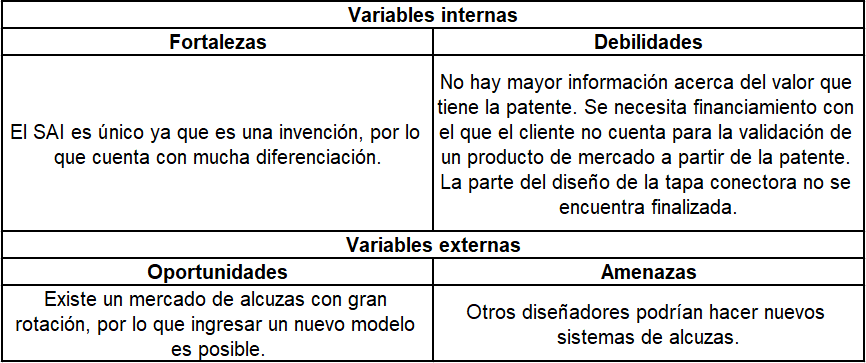
\includegraphics{FODA.png}
  \caption{Análisis FODA del proyecto de venta del SAI.}
  \label{foda1}
\end{figure}

Similarmente se realizó un análisis de las 5 fuerzas de Porter, el cual se detalla en la figura \ref{porter1}. Se ve a partir de esto, que el producto contiene un alto grado de diferenciación, pero existe una gran variedad de alcuzas tradicionales y no tradicionales disponibles en la competencia.

\begin{figure}
  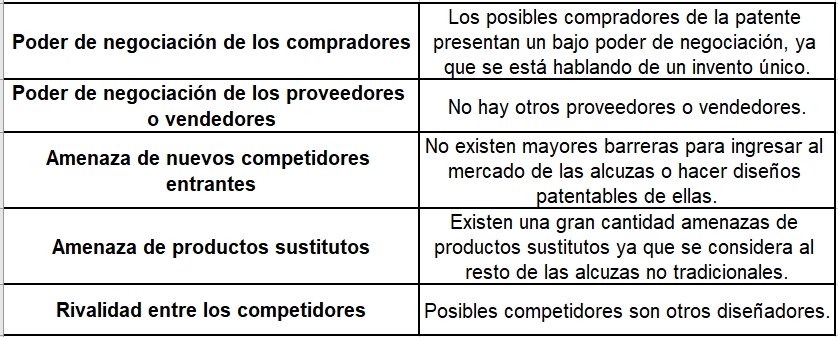
\includegraphics{Porter.png}
  \caption{Análisis de Porter del proyecto de venta del SAI.}
  \label{porter1}
\end{figure}

\subsection{Objetivos específicos de este trabajo}
\textbf{Objetivos Generales:}

Valorización de patente de invención de diseño de sistema de alcuza integrada INAPI registro N$^o$50.295 (22/10/2009)

Presentación de metodologías para la evaluación de patente de invención de diseño de sistema de alcuza integrada INAPI registro N$^o$50.295 (22/10/2009)



\textbf{Objetivos Específicos:}

Reducción de la incertidumbre en cuanto al precio de mercado que puede llegar a tener la patente INAPI  registro N$^o$50.295 (22/10/2009) para una posterior venta de los derechos de ella

Aumentar el marco de referencia que apoye la venta de patente de invención de diseño de sistema de alcuza integrada INAPI registro N$^o$50.295 (22/10/2009)
